\clearpage{}

\section{Define software requirements. Discuss means and stakeholders of
requirements elicitation. Describe the different types of requirements and
their desired characteristics. Explain and distinguish the nature of
requirements definition and specification documents.}

\subsection{Software requirements}



A requirement is an expression of desired behaviour which deals with objects or
entities, the states they can be in, and the functions that are performed to change states or
object characteristics. 
$\Rightarrow$ We are looking for requirements that identify key entities, limit
entities or define relationships among entities.
\newline

Focus on the customer needs (=\textit{what}), not implementation (=
\textit{how}). Incomplete requirements are one of the \textbf{top
factor for project failure}.

\subsubsection{The requirements process}

\begin{figure}[!ht]
    \centering
    \begin{tikzpicture}
        \small
        \node[draw, text width=2.2cm, align=center, minimum height=1cm] (Elicitation) {Elicitation};
        \node[draw, right = 1cm of Elicitation, text width=2.2cm, align=center, minimum height=1cm] (Analysis) {Analysis};
        \node[draw, right = 1cm of Analysis, text width=2.2cm, align=center, minimum height=1cm] (Specification) {Specification};
        \node[draw, right = 1cm of Specification, text width=2.2cm, align=center, minimum height=1cm] (Validation) {Validation};
        \node[draw, right = 1cm of Validation, text width=2.2cm, align=center, minimum height=1cm] (SRS) {Software Requirements Specification (SRS)};
        \node[below = 0.3cm of Elicitation, text width=3cm, align=center] {Collecting the user's requirements};
        \node[below = 0.3cm of Analysis, text width=3cm, align=center] {Understanding and modelling the desired behavior};
        \node[below = 0.3cm of Specification, text width=3cm, align=center] {Documenting the behavior of the proposed software system};
        \node[below = 0.3cm of Validation, text width=3cm, align=center] {Checking that our specification matches the user's requirements};
        \node[draw, fill=gray!50!white, right = 0.3cm of Validation, minimum height=4cm] {};

        \path[->, >=stealth] (Elicitation) edge node {} (Analysis);
        \path[->, >=stealth] (Analysis) edge node {} (Specification);
        \path[->, >=stealth] (Specification) edge node {} (Validation);
        \path[->, >=stealth] (Validation) edge node {} (SRS);
        \path[->, >=stealth] (Analysis) edge [out=75, in=75, looseness=0.7] node {} (Elicitation);
        \path[->, >=stealth] (Validation) edge [out=110, in=110, looseness=0.5] node {} (Elicitation);
    \end{tikzpicture}
    \caption{The requirement process}
\end{figure}
\FloatBarrier{}

More than simply writing down requirement: handle conflicts ($\neq$
point of view) to reach an agreement.
\newline

In agile method, requirements defined incrementally, essential requirements first,
additional requirements in subsequent releases.

\subsection{Requirements elicitation}

Collecting what the customers (and users) want from the system to be developed.
Need to discuss the requirements with everyone who has a stake in the system.

\textbf{Difficult} task 

\subsubsection{Stakeholders}

\begin{description}
    \item[Clients] paying for the software to be developed.
    \item[Customers] buying the software after it is developed.
    \item[Users] familiar with the current system and will use the future system.
    \item[Requirement Analyst] Determine the requirements
    \item[Domain experts] familiar with the problem that the software must automate.
    \item[Market researchers] have conducted surveys to determine future trends and potential customer’s needs.
    \item[Lawyers or auditors] familiar with government, safety or legal requirements.
    \item[Software engineers or other technology experts] ensure that the product is technically and economically feasible.
\end{description}

\begin{figure}[!ht]
    \centering
    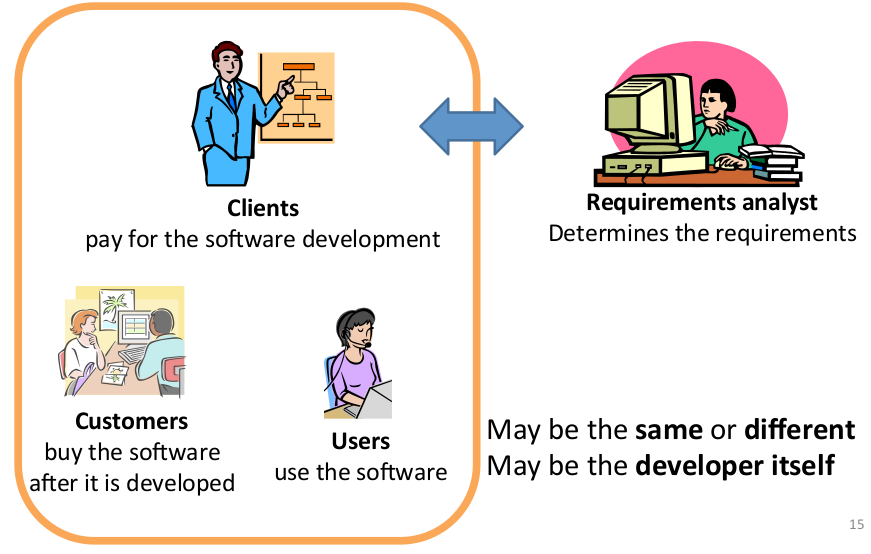
\includegraphics[width=0.4\linewidth]{elicitation1.png}
    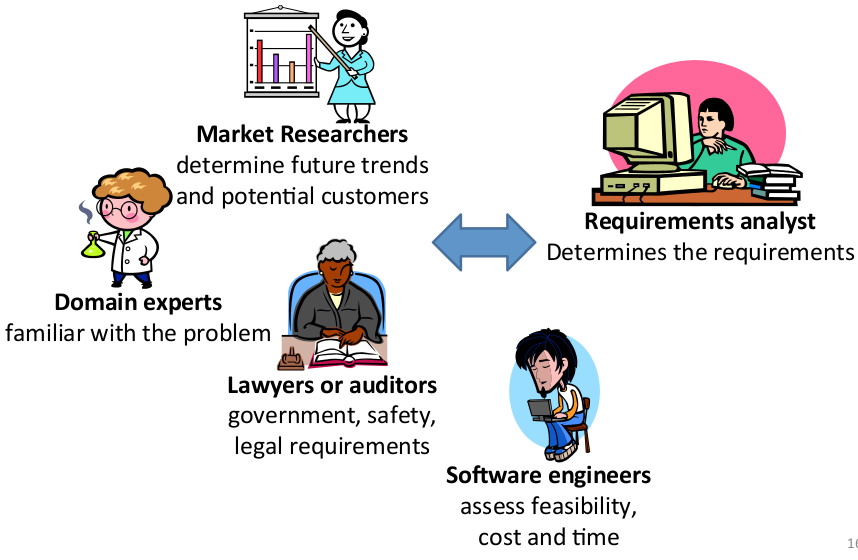
\includegraphics[width=0.4\linewidth]{elicitation2.png}
\end{figure}


Different skateholders have different view (may be inconsistent/conflict), so requirements need to be
presented in different way and agree on a compromise.

\subsubsection{Means}

\begin{figure}[!ht]
    \centering
    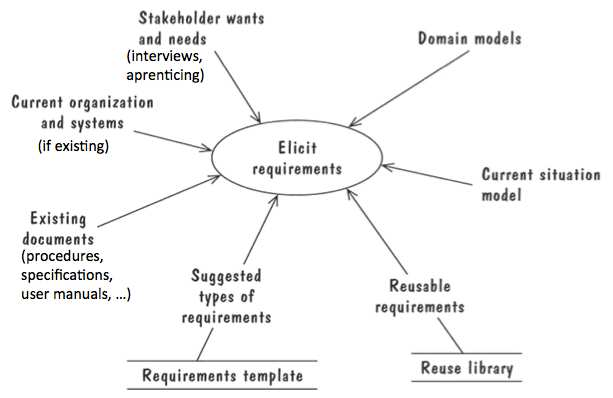
\includegraphics[width=0.4\linewidth]{requirement_process_means.png}
    \caption{Means of the requirements elicitation}
\end{figure}

You have to discuss with the stakeholder in group, to be inspired by other’s ideas. Different
stakeholder have different views, they can lead to inconsistencies. First, prioritize the
requirements:
\begin{itemize}
	\item must have / should have / could have / won't have
	\item essential / desirable/optional
\end{itemize}

Try to reach a compromise. Second, use the view points, in other words
don’t resolve inconsistencies early, keep just separate viewpoints and solve it later when
there is sufficient information.

\subsection{Types of requirements and their desired characteristics}

\begin{itemize}
    \item \textbf{Functional requirement:}
        It describes a required behaviour in terms of required activities, such as reactions to inputs,
        and the state of each entity before and after an activity occurs.

    \item \textbf{Quality (or nonfunctional) requirement:}
        It describes some required quality characteristic such as fast response time, ease of use,
        high reliability, low maintenance costs,\ldots

    \item \textbf{Design constraint:}
        It is an imposed design decision such as choice of platform or interface components.

    \item \textbf{Process constraint:}
        It is an imposed restriction on the techniques or resources to be used such as agile methods,
        prototypes,\ldots
\end{itemize}

\subsubsection{Desired qualities of the requirements:}

\begin{description}
    \item[Correct] the requirements conform to the desired understanding.
    \item[Consistent] all requirements can be satisfied simultaneously.
    \item[Unambiguous] requirements have a unique valid interpretation.
    \item[Complete] requirements specify the behaviour under all possible inputs, states and
contexts (externally) and define all terms (internally).
    \item[Feasible] it is possible to realize a system that meets all the requirements.
    \item[Relevant] all requirements correspond to desired or necessary functions or
characteristics.
    \item[Testable] it is possible to demonstrate whether every requirement is met.
    \item[Traceable] all requirements are labelled and organized for easy reference.
\end{description}

\subsection{Nature of requirements definition and specification documents}

\begin{figure}[!ht]
    \centering
    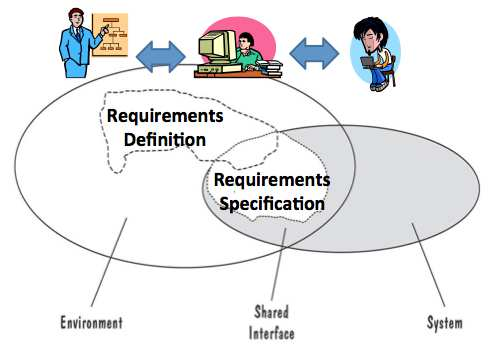
\includegraphics[width=0.4\linewidth]{requirements_documents.png}
    \caption{Two kinds of requirements documents}
\end{figure}
\FloatBarrier{}

\begin{itemize}

    \item \textbf{Software Requirements Definition (SRD):} Everything
        the customer wants to achieve, in terms of the environment of
        the system (i.e. expressed in the customer’s terms), aimed at a
        business audience, written by the client and the requirements
        analyst. 

        $\Rightarrow$ Its a record of the requirements expressed in the
        customer's terms.

        \begin{itemize}
            \item general purpose and scope 
            \item environment 
            \item characteristic of an acceptable solution
        \end{itemize}


\item \textbf{Software Requirements Specification (SRS):} A
    specification of how the proposed system shall behave, in terms of
    directly accessible environment (i.e.\ the boundary of the system),
    aimed at a technical audience, written by the requirements analyst
    for the developers.

    $\Rightarrow$  Restate the SRD in terms of the system’s interface,
    with sufficient details, without forcing a particular design.

    \begin{itemize}
            \item Quality requirement
            \item inputs/outputs in details (src, dst, protocols
                interaction, timing constraint,...)
                \end{itemize}

\end{itemize}


Note requirements traceability (correspondence between the different
development documents) is needed!
